\documentclass[border=10pt]{standalone}
\usepackage{tikz}
\usetikzlibrary{positioning,arrows.meta,shapes,fit,backgrounds,calc}

\begin{document}
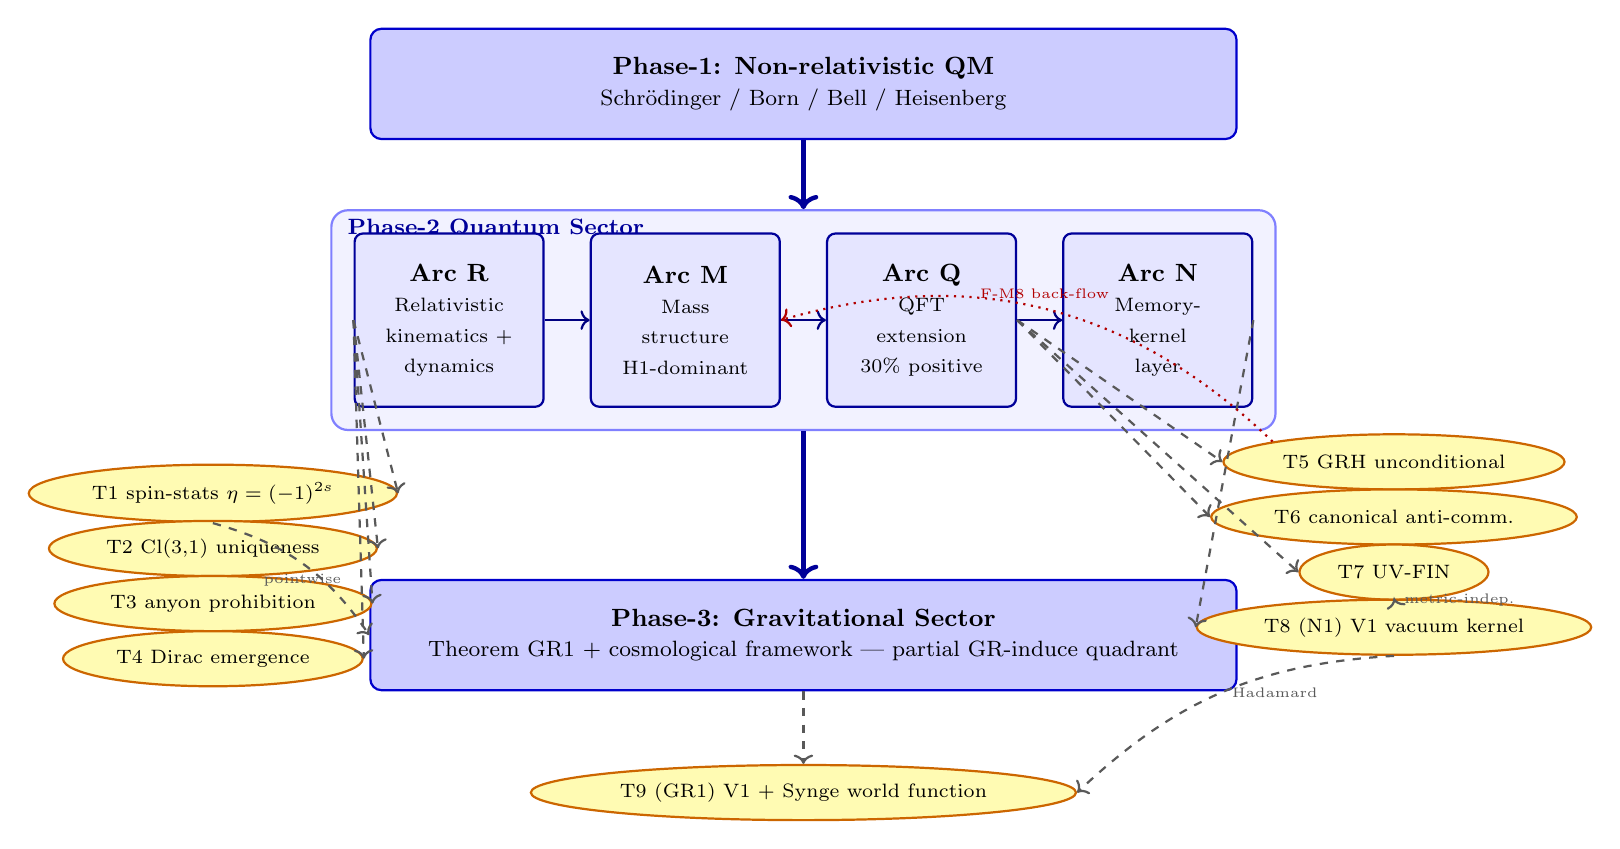
\begin{tikzpicture}[
    font=\small,
    phase/.style={rectangle, draw=blue!80!black, fill=blue!20, thick,
                  minimum width=11cm, minimum height=1.4cm, rounded corners=4pt,
                  align=center},
    arc/.style={rectangle, draw=blue!60!black, fill=blue!10, thick,
                minimum width=2.4cm, minimum height=2.2cm, rounded corners=3pt,
                align=center},
    thm/.style={ellipse, draw=orange!80!black, fill=yellow!30, thick,
                minimum width=2.4cm, minimum height=0.7cm, align=center,
                font=\scriptsize},
    flow/.style={->, ultra thick, blue!60!black},
    feed/.style={->, thick, gray!70!black, dashed},
    backflow/.style={->, thick, red!70!black, dotted}
]

% Phase-1 layer
\node[phase] (P1) at (0,0) {%
    \textbf{Phase-1: Non-relativistic QM}\\
    \footnotesize Schr\"odinger / Born / Bell / Heisenberg};

% Phase-2 four arcs
\node[arc] (AR) at (-4.5,-3) {\textbf{Arc R}\\\scriptsize Relativistic\\\scriptsize kinematics +\\\scriptsize dynamics};
\node[arc] (AM) at (-1.5,-3) {\textbf{Arc M}\\\scriptsize Mass\\\scriptsize structure\\\scriptsize H1-dominant};
\node[arc] (AQ) at (1.5,-3)  {\textbf{Arc Q}\\\scriptsize QFT\\\scriptsize extension\\\scriptsize 30\% positive};
\node[arc] (AN) at (4.5,-3)  {\textbf{Arc N}\\\scriptsize Memory-\\\scriptsize kernel\\\scriptsize layer};

% Phase-2 wrapper
\begin{scope}[on background layer]
    \node[draw=blue!50, fill=blue!5, thick, rounded corners=6pt,
          fit=(AR)(AM)(AQ)(AN), inner sep=8pt] (P2box) {};
    \node[anchor=north west, font=\bfseries\footnotesize, blue!60!black]
        at (P2box.north west) {\;Phase-2 Quantum Sector};
\end{scope}

% Phase-3 layer
\node[phase] (P3) at (0,-7) {%
    \textbf{Phase-3: Gravitational Sector}\\
    \footnotesize Theorem GR1 + cosmological framework
                  --- partial GR-induce quadrant};

% Theorems --- Arc R (T1-T4)
\node[thm] (T1) at (-7.5,-5.2) {T1 spin-stats $\eta=(-1)^{2s}$};
\node[thm] (T2) at (-7.5,-5.9) {T2 Cl(3,1) uniqueness};
\node[thm] (T3) at (-7.5,-6.6) {T3 anyon prohibition};
\node[thm] (T4) at (-7.5,-7.3) {T4 Dirac emergence};

% Theorems --- Arc Q (T5-T7)
\node[thm] (T5) at (7.5,-4.8) {T5 GRH unconditional};
\node[thm] (T6) at (7.5,-5.5) {T6 canonical anti-comm.};
\node[thm] (T7) at (7.5,-6.2) {T7 UV-FIN};

% Theorems --- Arc N (T8) and Phase-3 (T9)
\node[thm] (T8) at (7.5,-6.9) {T8 (N1) V1 vacuum kernel};
\node[thm] (T9) at (0,-9) {T9 (GR1) V1 + Synge world function};

% Phase flow (vertical layered)
\draw[flow] (P1) -- (P2box.north);
\draw[flow] (P2box.south) -- (P3);

% Inter-arc flow (within Phase-2)
\draw[->, thick, blue!50!black] (AR) -- (AM);
\draw[->, thick, blue!50!black] (AM) -- (AQ);
\draw[->, thick, blue!50!black] (AQ) -- (AN);

% Arc-to-theorem feeds
\draw[feed] (AR.west) -- (T1.east);
\draw[feed] (AR.west) -- (T2.east);
\draw[feed] (AR.west) -- (T3.east);
\draw[feed] (AR.west) -- (T4.east);
\draw[feed] (AQ.east) -- (T5.west);
\draw[feed] (AQ.east) -- (T6.west);
\draw[feed] (AQ.east) -- (T7.west);
\draw[feed] (AN.east) -- (T8.west);
\draw[feed] (P3.south) -- (T9.north);

% Cross-layer constraints (theorem → downstream)
\draw[feed, bend right=15] (T7.south) to node[midway,right,font=\tiny]
    {metric-indep.} (T8.north);
\draw[feed, bend right=20] (T8.south) to node[midway,right,font=\tiny]
    {Hadamard} (T9.east);
\draw[feed, bend left=20] (T1.south) to node[midway,below,font=\tiny]
    {pointwise} (P3.west);

% Back-flow: GRH → F-M8 in Arc M
\draw[backflow, bend right=30] (T5.north west) to node[midway,above,font=\tiny]
    {F-M8 back-flow} (AM.east);

\end{tikzpicture}
\end{document}
